\documentclass[10pt]{jhwhw}
\author{Ian Malerich}
\title{Math S 373: Homework 1}
\usepackage{amssymb, amsfonts, amsmath, mathtools, graphicx, breqn, soul}
\usepackage{minted, subfig, float, scrextend, setspace, amsthm}
\usemintedstyle{friendly}

\begin{document}
\raggedright

%% Problem 1
\problem{}

	\begin{enumerate}
		\item Show that $x-(\ln x)^x = 0$ has at least one solution on $[4,5]$.
		\item Use the Intermediate Value Theorem and Rolle's Theorem to show that the graph
			of $f(x) = x^3 + 2x + k$ crosses the x-axis exactly once, 
			regardless of the value of the constant k.
	\end{enumerate}

\solution

\part

	\begin{proof}
		Note that the function is continuous, in particular, it is continuous over $[4,5]$.
		Further as we have that 
		$f(4) = 4 - ln(4)^4 = 0.306638422$ and $f(5) = 5 - ln(5)^5 = -5.798691578$, and
		$-5.79869 < 0 < 0.306638422$, then by the Intermediate Value Theorem, 
		$\exists x\in[4,5] \text{ such that }
		f(x) = 0$.
	\end{proof}

\part

	\begin{proof}
		Note that as $f$ is a polynomial, thus it is continuous everywhere. In
		particular, it is continuous on any interval $(i,j)$ where $i,j \in \mathbb{R}$.
		\bigbreak
		If $x < 0$ then $x^3 + 2x + k < 2x + k$ further, if $x < -\frac{k}{2}$ then 
		$x^3 + 2x + k < 2x + k < 0$. \\ 
		Choose $a \in \mathbb{R}$ such that $a < -\frac{k}{2}$.
		\bigbreak
		If $x > 0$ then $x^3 + 2x + k > 2x + k$ further, if $x > -\frac{k}{2}$ then
		$x^3 + 2x + k > 2x + k > 0$. \\
		Choose $b \in \mathbb{R}$ such that $b > -\frac{k}{2}$.
		\bigbreak
		We know that $f$ is continuous on $(a,b)$, we also know that $f(a) < 0 < f(b)$. \\
		Thus, by the Intermediate Value Theorem, $\exists c\in(a,b) \text{ such that }
		f(c) = 0$.
	\end{proof}

%% Problem 2
\problem{}

	Let $f(x) = 2x\cos (2x) - (x-2)^2 \text{ and } x_0 = 0$.
	\begin{enumerate}
		\item Find the third Taylor polynomial $P_3(x)$, and use it to approximate $f(0.4)$
		\item Use the error formula in Taylor's Theorem to find an upper bound for the error
			$|f(0.4) - P_3(0.4)|$. Compute the actual error.
	\end{enumerate}

\solution

\part

	$P_3(x) = f(x_0) + f'(x_0)(x-x_0) + \frac{f''(x_0)}{2}(x-x_0)^2 + \frac{f^{(3)}(x_0)}{6}(x-x_0)^3$
	\begin{align*}
		f(0) = 2\times 0\cos (0) - (-2)^2 = -&4 \\
		f'(0) = -2x - 4x\sin (2x) + 2\cos (2x) + 4 = 2\cos 0 + 4 = 2 + 4 =\ &6 \\
		f''(0) = -2(4\sin (2x) + 4x\cos (2x) + 1) = -2(0 + 0 + 1) = -&2 \\
		f^{(3)}(0) = 8(2x\sin (2x) - 3\cos (2x)) = 8(0 - 3) = -&24
	\end{align*}

	Thus, the third Taylor polynomial about $x_0 = 0$ is given by
	$$
		P_3(x) = -4 + 6x + -x^2 + -4x^3
	$$
	Then
	$$
		f(0.4) \approx P_3(0.4) = -2.016
	$$

\part

	We have that $f^{(4)}(x) = 32(2\sin (2x) + x\cos (2x))$. \\
	The error is then given by the following (for some $c_x \in (0,0.4)$):
	$$
		\mathcal{E} (x) = \frac{f^{(4)}(c_x)}{24}x^4
	$$
	Thus, to find an upper bound of the error, we must find an upper bound for $f^{(4)}(c_x)$.
	This is found at $f^{(4)}(0.4) = 54.8286$. Giving us an error of 
	$\frac{54.8286}{24}(0.4)^4 = 0.05848384$.

	Actual error is given by $|f(0.4) - P_3(0.4)| = |-2.00263 - -2.016| = 0.0133654$.

%% Problem 3
\problem{}

	Let $f \in C[a,b]$ be a function whose derivative exists on $(a,b)$. Suppose $f$ is to be evaluated
	at $x_0$ in $(a,b)$, but instead of computing the actual value $f(x_0)$, the approximation value,
	$\widetilde{f}(x_0)$, is the actual value of $f$ at $x_0 + \epsilon$, that is 
	$\widetilde{f}(x_0) = f(x_0 + \epsilon)$.

	\begin{enumerate}
		\item Use the Mean Value Theorem to estimate the absolute error $|f(x_0) - \widetilde{f}(x_0)|$
			and the relative error $|f(x_0) - \widetilde{f}(x_0)|/|f(x_0)|$, assuming $f(x_0) \neq 0$.
		\item If $\epsilon = 5 \times 10^{-6}$ and $x_0=1$, find bounds for the absolute and relative errors for
			\begin{enumerate}
				\item $f(x) = e^x$
				\item $f(x) = \sin x$
			\end{enumerate}
	\end{enumerate}

\solution

\part 

	For absolute error, we have $|f(x_0) - \widetilde{f}(x_0)| = |f(x_0) - f(x_0+\epsilon)|$ by
	the mean value theorem it follows that
	$|f(x_0) - f(x_0+\epsilon)| = |f'(c)\epsilon|, c \in (x_0, x_0 + \epsilon)$. \\
	Therefore, our bound for absolute error is given by
	$\epsilon\times\sup|\{f'(c) : c\in (x_0,x_0+\epsilon)\}|$. \\
	Similarly, the bound for relative error is thus given by
	$\epsilon\times\sup|\{f'(c) : c\in (x_0,x_0+\epsilon)\}| / |f(x_0)|$.

\part

\textbf{(i)} $f(x) = e^x$

	To find absolute error by the formula given in part (a), we simply need to find the maximum
	derivative of $f(x)$ over $(1, 1 + 5\times10^{-6})$. As $e^x$ is non-decreasing, and $e^x' = e^x$
	the maximum is given by $e^{(1+5\times 10^{-6})} \approx 2.7182954199$ we then multiply this by $\epsilon$ to
	get the absolute error = $e^{1+5\times 10^{-6}}5\times 10^{-6} \approx 0.000013591477$.
	\bigbreak
	Relative error is then $(e^{1+5\times 10^{-6}}5\times 10^{-6})/(e^1) \approx 5.000025\times 10^{-6}$.

\bigbreak
\textbf{(ii)} $f(x) = \sin x$

	$f'(x) = \cos(x)$, thus to determine bound for absolute error, I need the maximum value
	of $\cos(x)$ over $(1, 1+5\times 10^{-6})$. Between 0 and $\pi/2\, \cos(x)$ is positive
	and decreasing. As we have $0 < 1 < 1+5\times 10^{-6} < \pi/2$ we will find our maximum value
	at $cos(1) \approx 0.5403023$. We then multiply this by $\epsilon$ to get the absolute error
	= $\cos(1)\times\epsilon \approx 2.701511529\times10^{-6}$.
	\bigbreak
	Relative error is then $\cos(1)\times\epsilon/\sin(1) \approx 3.210463\times10^{-6}$.

%% Problem 4
\problem{}

	The equation $4x^2 - e^x - e^{-x} = 0$ has four solutions $\pm x_1$ and $\pm x_2$.
	Use Newton's method to approximate the solution to within $10^-5$ with the following values of
	$y_0: \text{(a)} p_0 = -10$, (b) $p_0 = -5$, (c) $p_0 = -3$, (d) $p_0 = -1$, (c) $p_0 = 1$, 
	(g) $p_0 = 3$, (h) $p_0 = 5$, (i) $p_0 = 10$. Comment on the results.

\solution

	\inputminted{octave}{p4.m}
	Below I have formatted the text output from that code, we can immediately see
	some symmetry about the axis $x=0$. Using the initial $y_0$ values, I found
	a total of 4 zeros at $x=\{\pm4.3062, \pm0.82450\}$.
	The closer I start to the guess, the faster (less steps) Newton's method will
	find a result. Interestingly, $x=\pm3$ overshoot the zero on their side
	of the axis $x=0$, that is $+3\text{ finds }-0.82450$ and $-3\text{ finds }+0.82450$.
	All others initial values find the zero nearest to them.

	\inputminted{text}{p4.results}

	\clearpage
	And here is a graph to visualize what Newton's method is doing for each starting point.
	Note there is some overlap for initial values of $\pm3$ as they approach
	opposite zeros.
	\begin{center}
		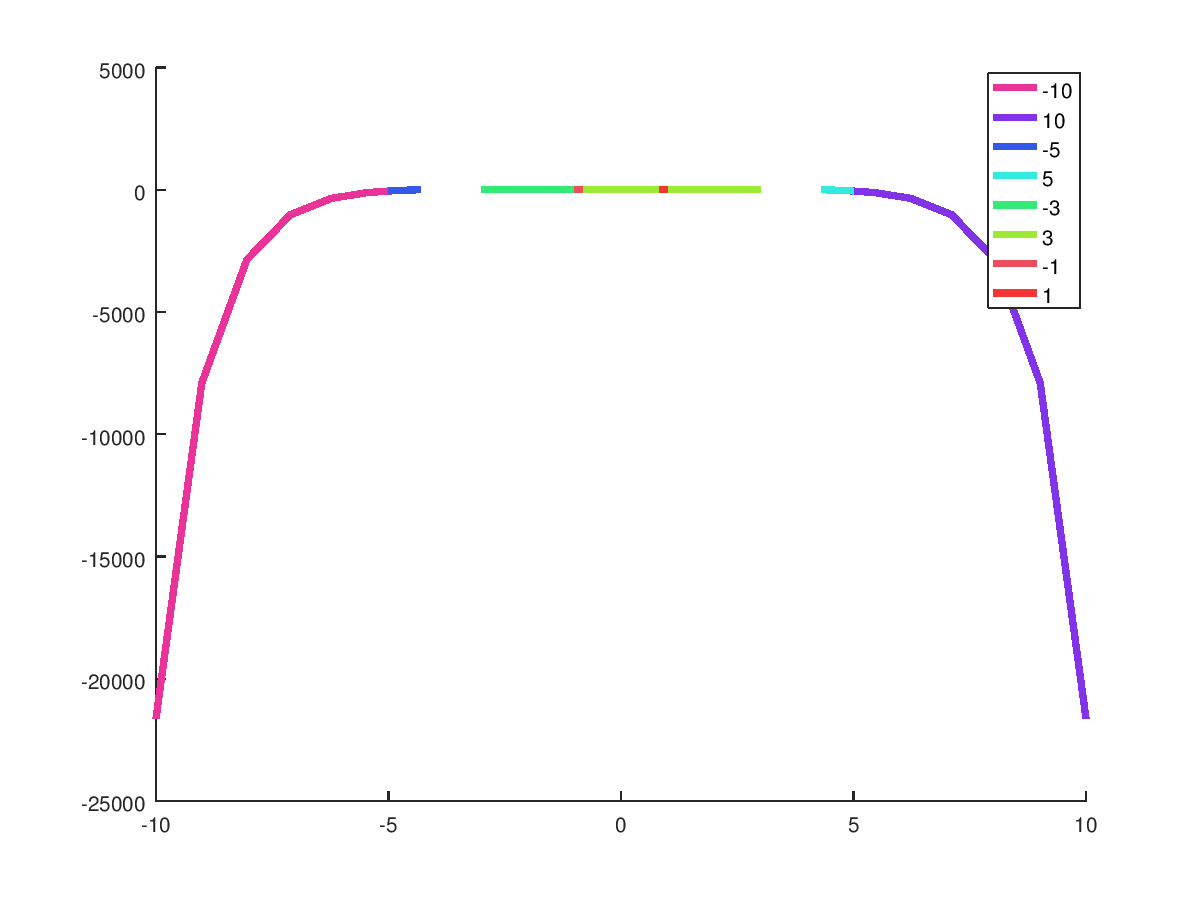
\includegraphics[scale=0.8]{p4.png}
	\end{center}

%% Problem 5
\problem{}

	Use Newton's method and Modified Newton's method to find the solution accurate to 
	within $10^{-5}$ for
	$$
		1 - 4x\cos x + 2x^2 + \cos 2x = 0\text{, for }0 \leq x \leq 1.
	$$
	Comment on the performance of the methods.

\solution

	\inputminted{octave}{p5.m}
	Here are the results we get from running regular \hl{Newton's Method} to find the zero.
	From the steps used to find the solution, we can see that Newton's method 
	took \hl{9 steps} when using the midpoint to find the zero.
	\inputminted{text}{p5.newtons}
	And here are the results when we use \hl{Modified Newton's Method} to find the zero.
	We can see that this method found a result much faster than regular Newton's Method, 
	taking only \hl{5 steps} to find the (more accurate) solution.
	\inputminted{text}{p5.modified}
	In the graph below, we can clearly see Modified Newton's Method jumping straight away
	from $0.5$ to $0.7$ in one step, something that regular Newton's Method took about 3 
	steps.
	\begin{center}
		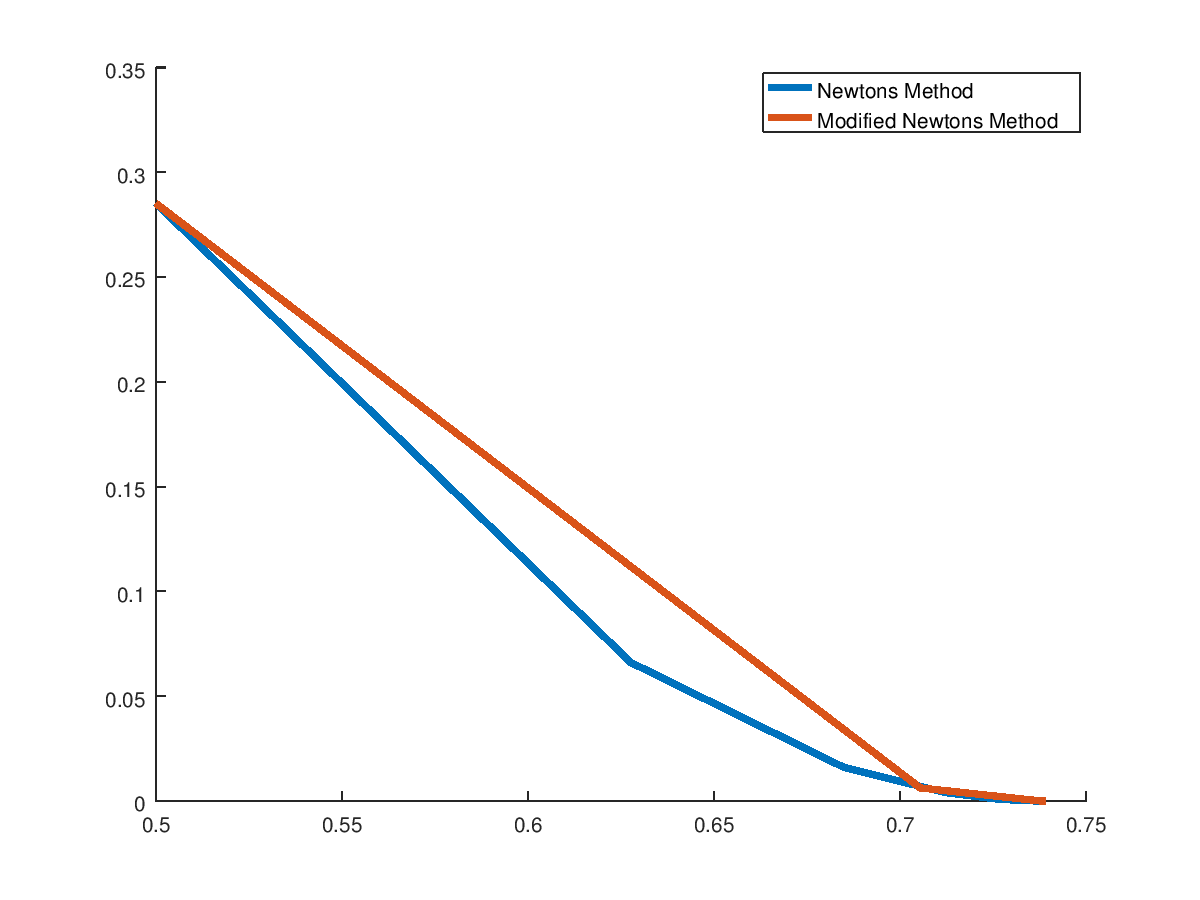
\includegraphics[scale=0.5]{p5.png}
	\end{center}

%% Problem 6
\problem{}

	Use each of the following methods to find a solution in $[0.1, 1]$ 
	accurate to within $10^-4$ for
	$$
		600x^4 - 550x^3 + 200x^2 - 20x - 1 = 0.
	$$
	\begin{enumerate}
		\item Bisection method
		\item Newton's method
		\item Secant method
		\item M\"{u}ller's method
	\end{enumerate}
	Comment on the performance of these methods.

\solution
	
	\inputminted{octave}{p6.m}
	\bigbreak
	\textcolor[RGB]{240,240,240}{\rule{\textwidth}{0.5pt}}\bigbreak
	\bigbreak

	The \hl{Bisection Method} is the slowest solution of these 4 methods, taking 
	a total of \hl{15 steps} to find a solution. Further, this solution only barely
	breaks the required error, indicative of the small jumps taken by this method.
	\inputminted{text}{p6.bisection}
	\textcolor[RGB]{240,240,240}{\rule{\textwidth}{0.5pt}}\bigbreak
	
	\hl{Newton's Method} is about twice as fast as the Bisection Method in this example,
	converging in just \hl{6 steps}. Likely due to the simplicity of finding the zero
	of a polynomial, with an initial guess that was relatively close to what we were looking
	for, that is, more complex methods were likely not needed in this scenario.
	\inputminted{text}{p6.newtons}

	\textcolor[RGB]{240,240,240}{\rule{\textwidth}{0.5pt}}\bigbreak
	The \hl{Secant Method} found a solution slightly slower than Newton's, taking
	an additional step, for a total of \hl{7 steps}. This does however, include 
	both of the initial guesses, one of which was derived from Newton's method.
	\inputminted{text}{p6.secant}
	\textcolor[RGB]{240,240,240}{\rule{\textwidth}{0.5pt}}\bigbreak

	\clearpage
	\hl{M\"uller's Method} found it's result in \hl{8 steps}, which included 3 initial
	guesses, 2 of which were found using Newton's method. If these Initial guesses are 
	excluded from the count, only 5 steps of iteration were actually needed. Which
	would bring tie it with Newton's method. Regardless, this method was not necessarily
	needed in finding the desired 0, although this function does have complex 0's,
	we did not actually find one using these initial parameters.
	\inputminted{text}{p6.muller}
	\textcolor[RGB]{240,240,240}{\rule{\textwidth}{0.5pt}}\bigbreak

	\begin{center}
		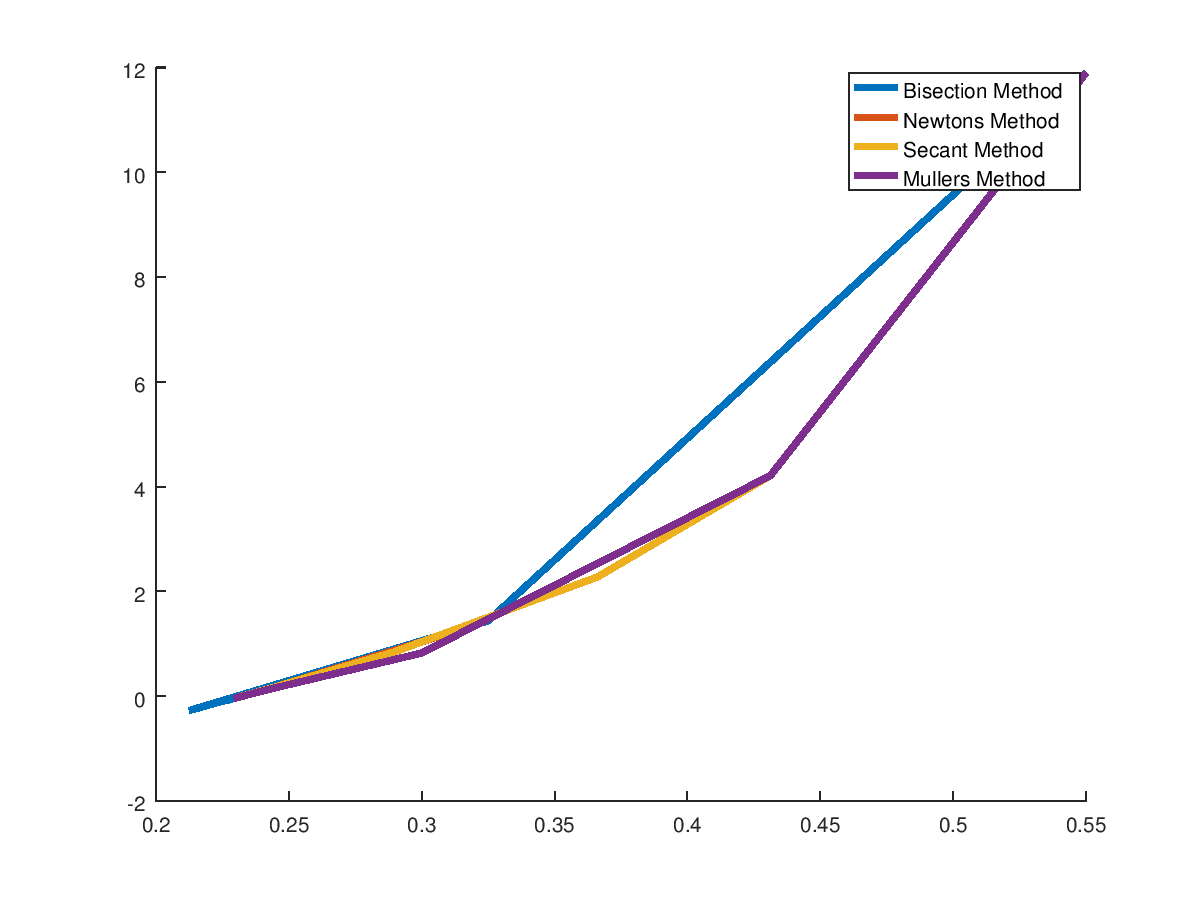
\includegraphics[scale=0.75]{p6.png}
	\end{center}

%% Problem 7
\problem{}

	An object falling vertically through the air is subjected to viscous resistance as well as the
	force of gravity. Assume that an object with mass $m$ is dropped from a height $s_0$ and that the height of the
	object after $t$ seconds is
	$$
		s(t) = s_0 - \frac{mg}{k}t + \frac{m^2g}{k^2}(1-e^{-kt/m}),
	$$
	where $g=32.17 ft/s^2$ and $k$ represents the coefficient of air resistance in lb-s/ft.
	Suppose $s_0$=300ft, $m$ = 0.25lb, and $k$ = 0.1 lb-s/ft. Find to within 0.01s the time it takes
	this quarter-pounder to hit the ground. Use Fixed-point iteration, Steffensen's method and Newton's method
	to find the solution.

\solution
	\inputminted{octave}{p7.m}
	\hl{Fixed-Point Iteration} was the slowest of the three methods I used, but thanks
	to a decent initial guess, and a relatively large error, none of the methods took
	particularly long to find a solution. In this case, only \hl{5 steps} were needed.
	\inputminted{text}{p7.fixedpoint}
	\textcolor[RGB]{240,240,240}{\rule{\textwidth}{0.5pt}}\bigbreak

	\hl{Steffensen's Method} found a solution in only \hl{3 steps}, just as fast as 
	Newton's method. However, Steffensen's method produced a notably much closer
	result, and had much greater accuracy than the other two methods.
	\inputminted{text}{p7.steffensens}
	\textcolor[RGB]{240,240,240}{\rule{\textwidth}{0.5pt}}\bigbreak

	Like Steffensen's Method, \hl{Newton's Method} found a solution in only
	\hl{3 steps}, however as noted above the result was not as accurate as the one
	found by Steffensen's Method, although the result was still better than
	Fixed-Point Iteration. This may have to do with the fact that the solution was
	found so quickly, and may not be indicative of long term behavior.
	\inputminted{text}{p7.newtons}
	\textcolor[RGB]{240,240,240}{\rule{\textwidth}{0.5pt}}\bigbreak
	
	In the graph below, we can see that although the number of steps varied,
	the path took in all these methods was roughly the same, this again is likely due to
	the initial guess being reasonably close to the desired solution.
	\begin{center}
		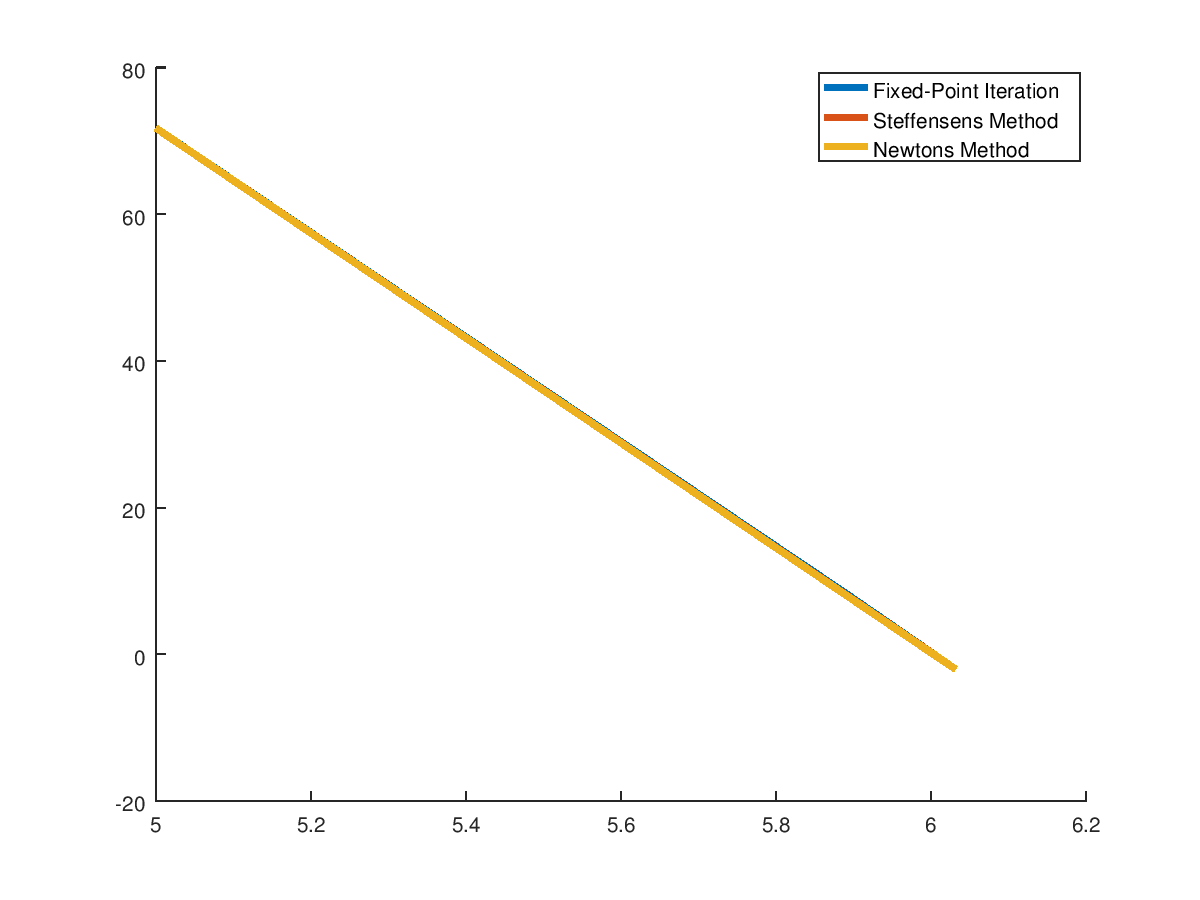
\includegraphics[scale=0.75]{p7.png}
	\end{center}

\end{document}
